\section{相关理论与技术基础}
\setchapternum{2}

本章简要介绍本文方法所依托的理论基础，包括人工神经网络与卷积神经网络的基本组成，以及实验所用的 MNIST 数据集。

\subsection{人工神经网络基础}

人工神经网络由大量神经元分层连接而成。单个神经元对输入 $x_1,\dots,x_n$ 加权求和并经激活函数 $f(\cdot)$ 输出，如式(\ref{eq:neuron})所示。网络参数通过反向传播算法\cite{rumelhart1986learning}与梯度下降进行训练。

% ===== 带编号公式示例（编号自动为「2-序号」）=====
\begin{equation}
a = f\!\left( \sum_{i=1}^{n} w_i x_i + b \right)
\label{eq:neuron}
\end{equation}

\subsection{卷积神经网络}

卷积神经网络针对图像数据引入局部连接、权值共享与下采样机制，能够自动学习由低级到高级的层次化特征，相比全连接网络大幅减少了参数量\cite{lecun1998gradient,goodfellow2016deep}。其典型结构由卷积层、池化层交替堆叠，最后接全连接层完成分类，如图\ref{fig:cnn-arch}所示。

% ===== 插图示例（图片放在 figures/ 目录；中英文图题用 \\ 换行）=====
\begin{figure}[htb]
\centering
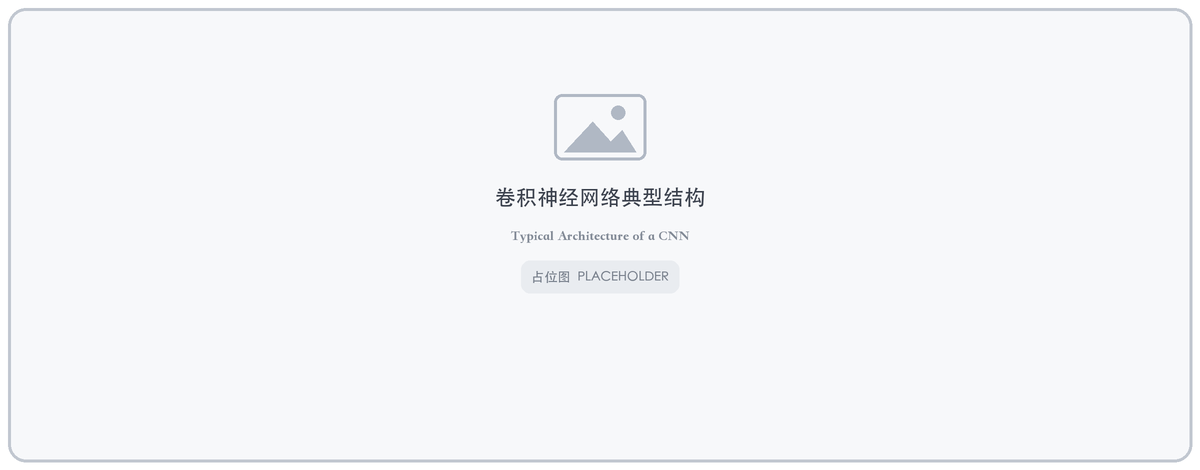
\includegraphics[width=0.95\linewidth]{figures/fig-cnn-architecture.png}
\caption{卷积神经网络典型结构\\Fig.~\thefigure\ Typical architecture of a convolutional neural network}
\label{fig:cnn-arch}
\end{figure}

\subsubsection{卷积层}

卷积层通过卷积核在输入特征图上滑动提取局部特征。设输入宽度为 $W$、卷积核大小为 $K$、填充为 $P$、步长为 $S$，则输出特征图宽度如式(\ref{eq:convsize})所示，高度同理。本文采用 $3\times3$ 卷积核并通过权值共享降低参数量。

\begin{equation}
W' = \frac{W - K + 2P}{S} + 1
\label{eq:convsize}
\end{equation}

\subsubsection{激活函数与池化}

为引入非线性，本文在卷积层后采用修正线性单元（ReLU）\cite{nair2010rectified}，其定义为 $f(x)=\max(0,x)$，可有效缓解梯度消失并加速收敛。池化层用于下采样，本文采用 $2\times2$ 最大池化，在保留显著特征的同时将特征图尺寸减半，并增强对微小位移的鲁棒性。

\subsection{MNIST 数据集}

MNIST 是手写数字识别领域应用最广的标准基准\cite{lecun1998gradient,deng2012mnist}，包含 $60{,}000$ 张训练图像与 $10{,}000$ 张测试图像，每张为 $28\times28$ 灰度图，对应 $0\sim9$ 共十个类别。

\subsection{本章小结}

本章梳理了人工神经网络与卷积神经网络的基本原理，并介绍了实验数据集，为后续网络设计与实验奠定基础。
